\documentclass[aspectratio=169]{beamer}
\mode<presentation>
%\usetheme{Warsaw}
%\usetheme{Goettingen}
\usetheme{Hannover}
%\useoutertheme{default}

%\useoutertheme{infolines}
\useoutertheme{sidebar}
\usecolortheme{dolphin}

\usepackage{amsmath}
\usepackage{amssymb}
\usepackage{enumerate}

%some bold math symbosl
\newcommand{\Cov}{\mathrm{Cov}}
\newcommand{\Cor}{\mathrm{Cor}}
\newcommand{\Var}{\mathrm{Var}}
\newcommand{\brho}{\boldsymbol{\rho}}
\newcommand{\bSigma}{\boldsymbol{\Sigma}}
\newcommand{\btheta}{\boldsymbol{\theta}}
\newcommand{\bbeta}{\boldsymbol{\beta}}
\newcommand{\bmu}{\boldsymbol{\mu}}
\newcommand{\bW}{\mathbf{W}}
\newcommand{\one}{\mathbf{1}}
\newcommand{\bH}{\mathbf{H}}
\newcommand{\by}{\mathbf{y}}
\newcommand{\bolde}{\mathbf{e}}
\newcommand{\bx}{\mathbf{x}}

\newcommand{\cpp}[1]{\texttt{#1}}

\title{Mathematical Biostatistics Boot Camp 2: Lecture 4, Two Sample Binomial Tests}
\author{Brian Caffo}
\date{\today}
\institute[Department of Biostatistics]{
  Department of Biostatistics \\
  Johns Hopkins Bloomberg School of Public Health\\
  Johns Hopkins University
}


\begin{document}
\frame{\titlepage}

%\section{Table of contents}
\frame{
  \frametitle{Table of contents}
  \tableofcontents
}

\begin{frame}\frametitle{Motivation}
  \begin{itemize}
  \item Consider a randomized trial where 40 subjects were randomized (20 each) to 
    two drugs with the same active ingredient but different expedients
  \item Consider counting the number of subjects with side effects for each drug
    \begin{center}
      \ttfamily
      \begin{tabular}{lccc}
        & Side    &      &       \\
        & Effects & None & total \\ \hline
        Drug A & 11           & 9    & 20 \\
        Drug B &  5           & 15   & 20 \\ \hline
        Total   & 16           & 14   & 40 
      \end{tabular}
      \normalfont
    \end{center}
  \end{itemize}
\end{frame}

\section{The score statistic}
\begin{frame}\frametitle{Hypothesis tests for binomial proportions}
  \begin{itemize}
  \item Consider testing $H_0:p=p_0$ for a binomial proportion
  \item The {\bf score} test statistic
    $$
    \frac{\hat p - p_0}{\sqrt{p_0(1 - p_0) / n}}
    $$
    follows a $Z$ distribution for large $n$
  \item This test performs better than the Wald test
    $$
    \frac{\hat p - p_0}{\sqrt{\hat p(1 - \hat p) / n}}
    $$
  \end{itemize}
\end{frame}

\begin{frame}\frametitle{Inverting the two intervals}
  \begin{itemize}
  \item Inverting the Wald test yields the Wald interval
    $$
    \hat p \pm Z_{1 - \alpha / 2} \sqrt{\hat p(1 - \hat p) / n}
    $$
  \item Inverting the Score test yields the Score interval
    \small
    \begin{eqnarray*}
      &  \hat p \left(\frac{n}{n + Z_{1 - \alpha / 2}^2}\right) + 
      \frac{1}{2} \left(\frac{Z_{1 - \alpha / 2}^2}{n + Z_{1 - \alpha / 2}^2}\right) \\\\ 
      &  \pm Z_{1 - \alpha/2}\sqrt{\frac{1}{n + Z_{1 - \alpha / 2}^2} 
        \left[\hat p (1 - \hat p) \left(\frac{n}{n + Z_{1 - \alpha / 2}^2}\right) +
          \frac{1}{4} \left(\frac{Z_{1 - \alpha / 2}^2}{n + Z_{1 - \alpha / 2}^2}\right)
        \right]}
    \end{eqnarray*}
    \normalsize
  \item Plugging in $Z_{1-\alpha / 2} = 2$ yields the Agresti/Coull interval
  \end{itemize}
\end{frame}

\begin{frame}\frametitle{Example}
  \begin{itemize}
  \item In our previous example consider testing whether or not Drug A's
    percentage of subjects with side effects is greater than 10\%
  \item $H_0 : p_A = .1$ verus $H_A : p_A > .1$ 
  \item $\hat p = 11 / 20 = .55$
  \item Test Statistic $$\frac{.55 - .1}{\sqrt{.1 \times .9 / 20}} = 6.7$$
  \item Reject, pvalue = $P(Z > 6.7) \approx 0$
  \end{itemize}
\end{frame}

\section{Exact tests}
\begin{frame}\frametitle{Exact binomial tests} 
  \begin{itemize}
  \item Consider calculating an exact P-value
  \item What's the probability, under the null hypothesis, of getting
    evidence as extreme or more extreme than we obtained?
    $$P(X_A \geq 11) = 
    \sum_{x=11}^{20}\left(\begin{array}{c}20 \\ x \end{array}\right) .1^x\times .9^{20-x}
    \approx 0
    $$
  \item \texttt{pbinom(10, 20, .1, lower.tail = FALSE)}
  \item \texttt{binom.test(11, 20, .1, alternative = "greater")}
  \end{itemize}
\end{frame}

\begin{frame}\frametitle{Notes on exact binomial tests}
  \begin{itemize}
  \item This test, unlike the asymptotic ones, guarantees the Type I error rate
    is less than desired level; sometimes it is much less
  \item Inverting the exact binomial test yields an exact binomial
    interval for the true proprotion 
  \item This interval (the Clopper/Pearson interval) has coverage greater
    than 95\%, though can be very conservative
  \item For two sided tests, calculate the two one sided P-values and double the
    smaller
  \end{itemize}
\end{frame}

\begin{frame}\frametitle{Wald versus Agresti / Coull\footnote{Taken from Agresti and Caffo (2000) TAS }}
\begin{center}
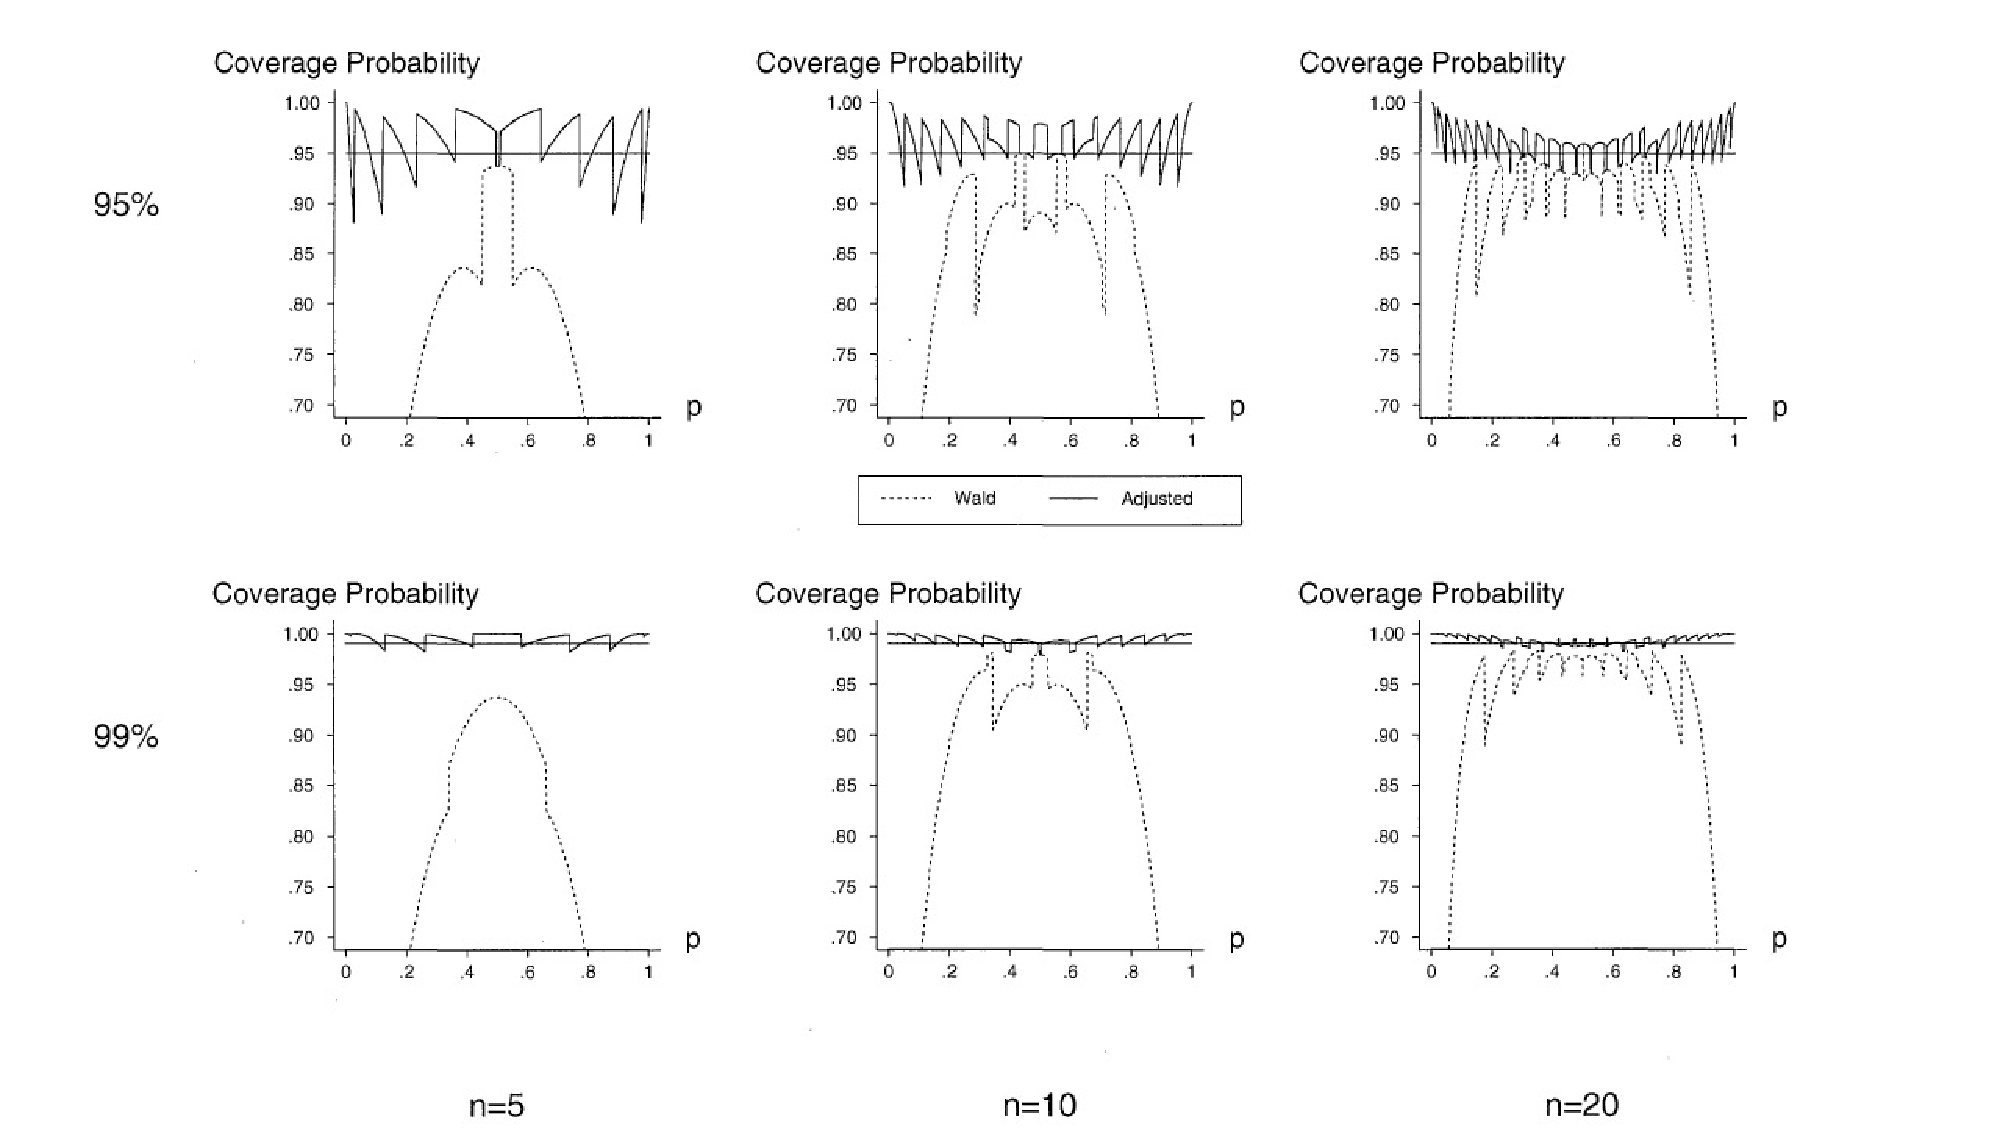
\includegraphics[width=4in]{waldCoverage.pdf}
\end{center}
\end{frame}

\section{Comparing two binomial proportions}
\begin{frame}\frametitle{Comparing two binomials}
  \begin{itemize}
  \item Consider now testing whether the proportion of side effects is the same
    in the two groups
  \item Let $X \sim \mathrm{Binomial}(n_1, p_1)$ and $\hat p_1 = X / n_1$
  \item Let $Y \sim \mathrm{Binomial}(n_2, p_2)$ and $\hat p_2 = Y / n_2$
  \item We also use the following notation:
    \begin{center}
      \begin{tabular}{|c|c|c|}\hline
        $n_{11} = X$ & $n_{12} = n_1 - X$ & $n_1 = n_{1+}$ \\ \hline
        $n_{21} = Y$ & $n_{22} = n_2 - Y$ & $n_2 = n_{2+}$ \\ \hline
        $n_{+1}$     & $n_{+2}$           &       \\ \hline 
      \end{tabular}
    \end{center}
  \end{itemize}
\end{frame}

\begin{frame}\frametitle{Comparing two proportions}
  \begin{itemize}
  \item Consider testing $H_0:p_1 = p_2$ 
  \item Versus $H_1:p_1 \neq p_2$, $H_2:p_1>p_2$, $H_3:p_1 < p_2$ 
  \item The score test statstic for this null hypothesis is
    $$
    TS = \frac{\hat p_1 - \hat p_2}{\sqrt{\hat p (1 - \hat p)(\frac{1}{n_1} + \frac{1}{n_2})}}
    $$
    where $\hat p = \frac{X + Y}{n_1 + n_2}$ is the estimate of the
    common proportion under the null hypothesis
  \item This statistic is normally distributed for large $n_1$ and
    $n_2$.
  \end{itemize}
\end{frame}

\begin{frame}\frametitle{Continued}
  \begin{itemize}
  \item This interval does not have a closed form inverse for creating a
    confidence interval (though the numerical interval obtained performs
    well)
  \item An alternate interval inverts the Wald test
    $$
    TS = \frac{\hat p_1 - \hat p_2}{\sqrt{\frac{\hat p_1 (1 - \hat p_1)}{n_1} + \frac{\hat p_2(1 - \hat p_2)}{n_2}}}
    $$
  \item The resulting confidence interval is
    $$
    \hat p_1 - \hat p_2 \pm Z_{1-\alpha / 2}\sqrt{\frac{\hat p_1 (1 - \hat p_1)}{n_1} + \frac{\hat p_2(1 - \hat p_2)}{n_2}}
    $$
    \end{itemize}
  \end{frame}

\begin{frame}\frametitle{Continued}
  \begin{itemize}
  \item As in the one sample case, the Wald interval and test performs poorly
    relative to the score interval and test
  \item For testing, always use the score test
  \item For intervals, inverting the score test is hard and not offered in standard software
  \item A simple fix is the Agresti/Caffo interval which is obtained by calculating $\tilde p_1 = \frac{x + 1}{n_1 + 2}$, $\tilde n_1 = n_1 + 2$, $\tilde p_2 = \frac{y + 1}{n_2 + 2}$ and $\tilde n_2 = (n_2 + 2)$
  \item Using these, simply construct the Wald interval  
  \item This interval does not approximate the score interval, but does
    perform better than the Wald interval
  \end{itemize}
\end{frame}
 

\begin{frame}\frametitle{Example} 
  \begin{itemize}
  \item Test whether or not the proportion of side effects is the same
    for the two drugs
  \item $\hat p_A = .55$, $\hat p_B = 5 / 20 = .25$, $\hat p = 16 / 40 = .4$
  \item Test statistic
    $$
    \frac{.55 - .25}{\sqrt{.4 \times .6 \times (1 / 20 + 1 / 20)}} = 1.61
    $$
  \item Fail to reject $H_0$ at $.05$ level (compare with $1.96$)
  \item P-value $P(|Z| \geq 1.61) = .11$
  \end{itemize}
\end{frame}

\begin{frame}\frametitle{Wald versus Agresti /Caffo\footnote{Taken from Agresti and Caffo (2000) TAS }}
\begin{center}
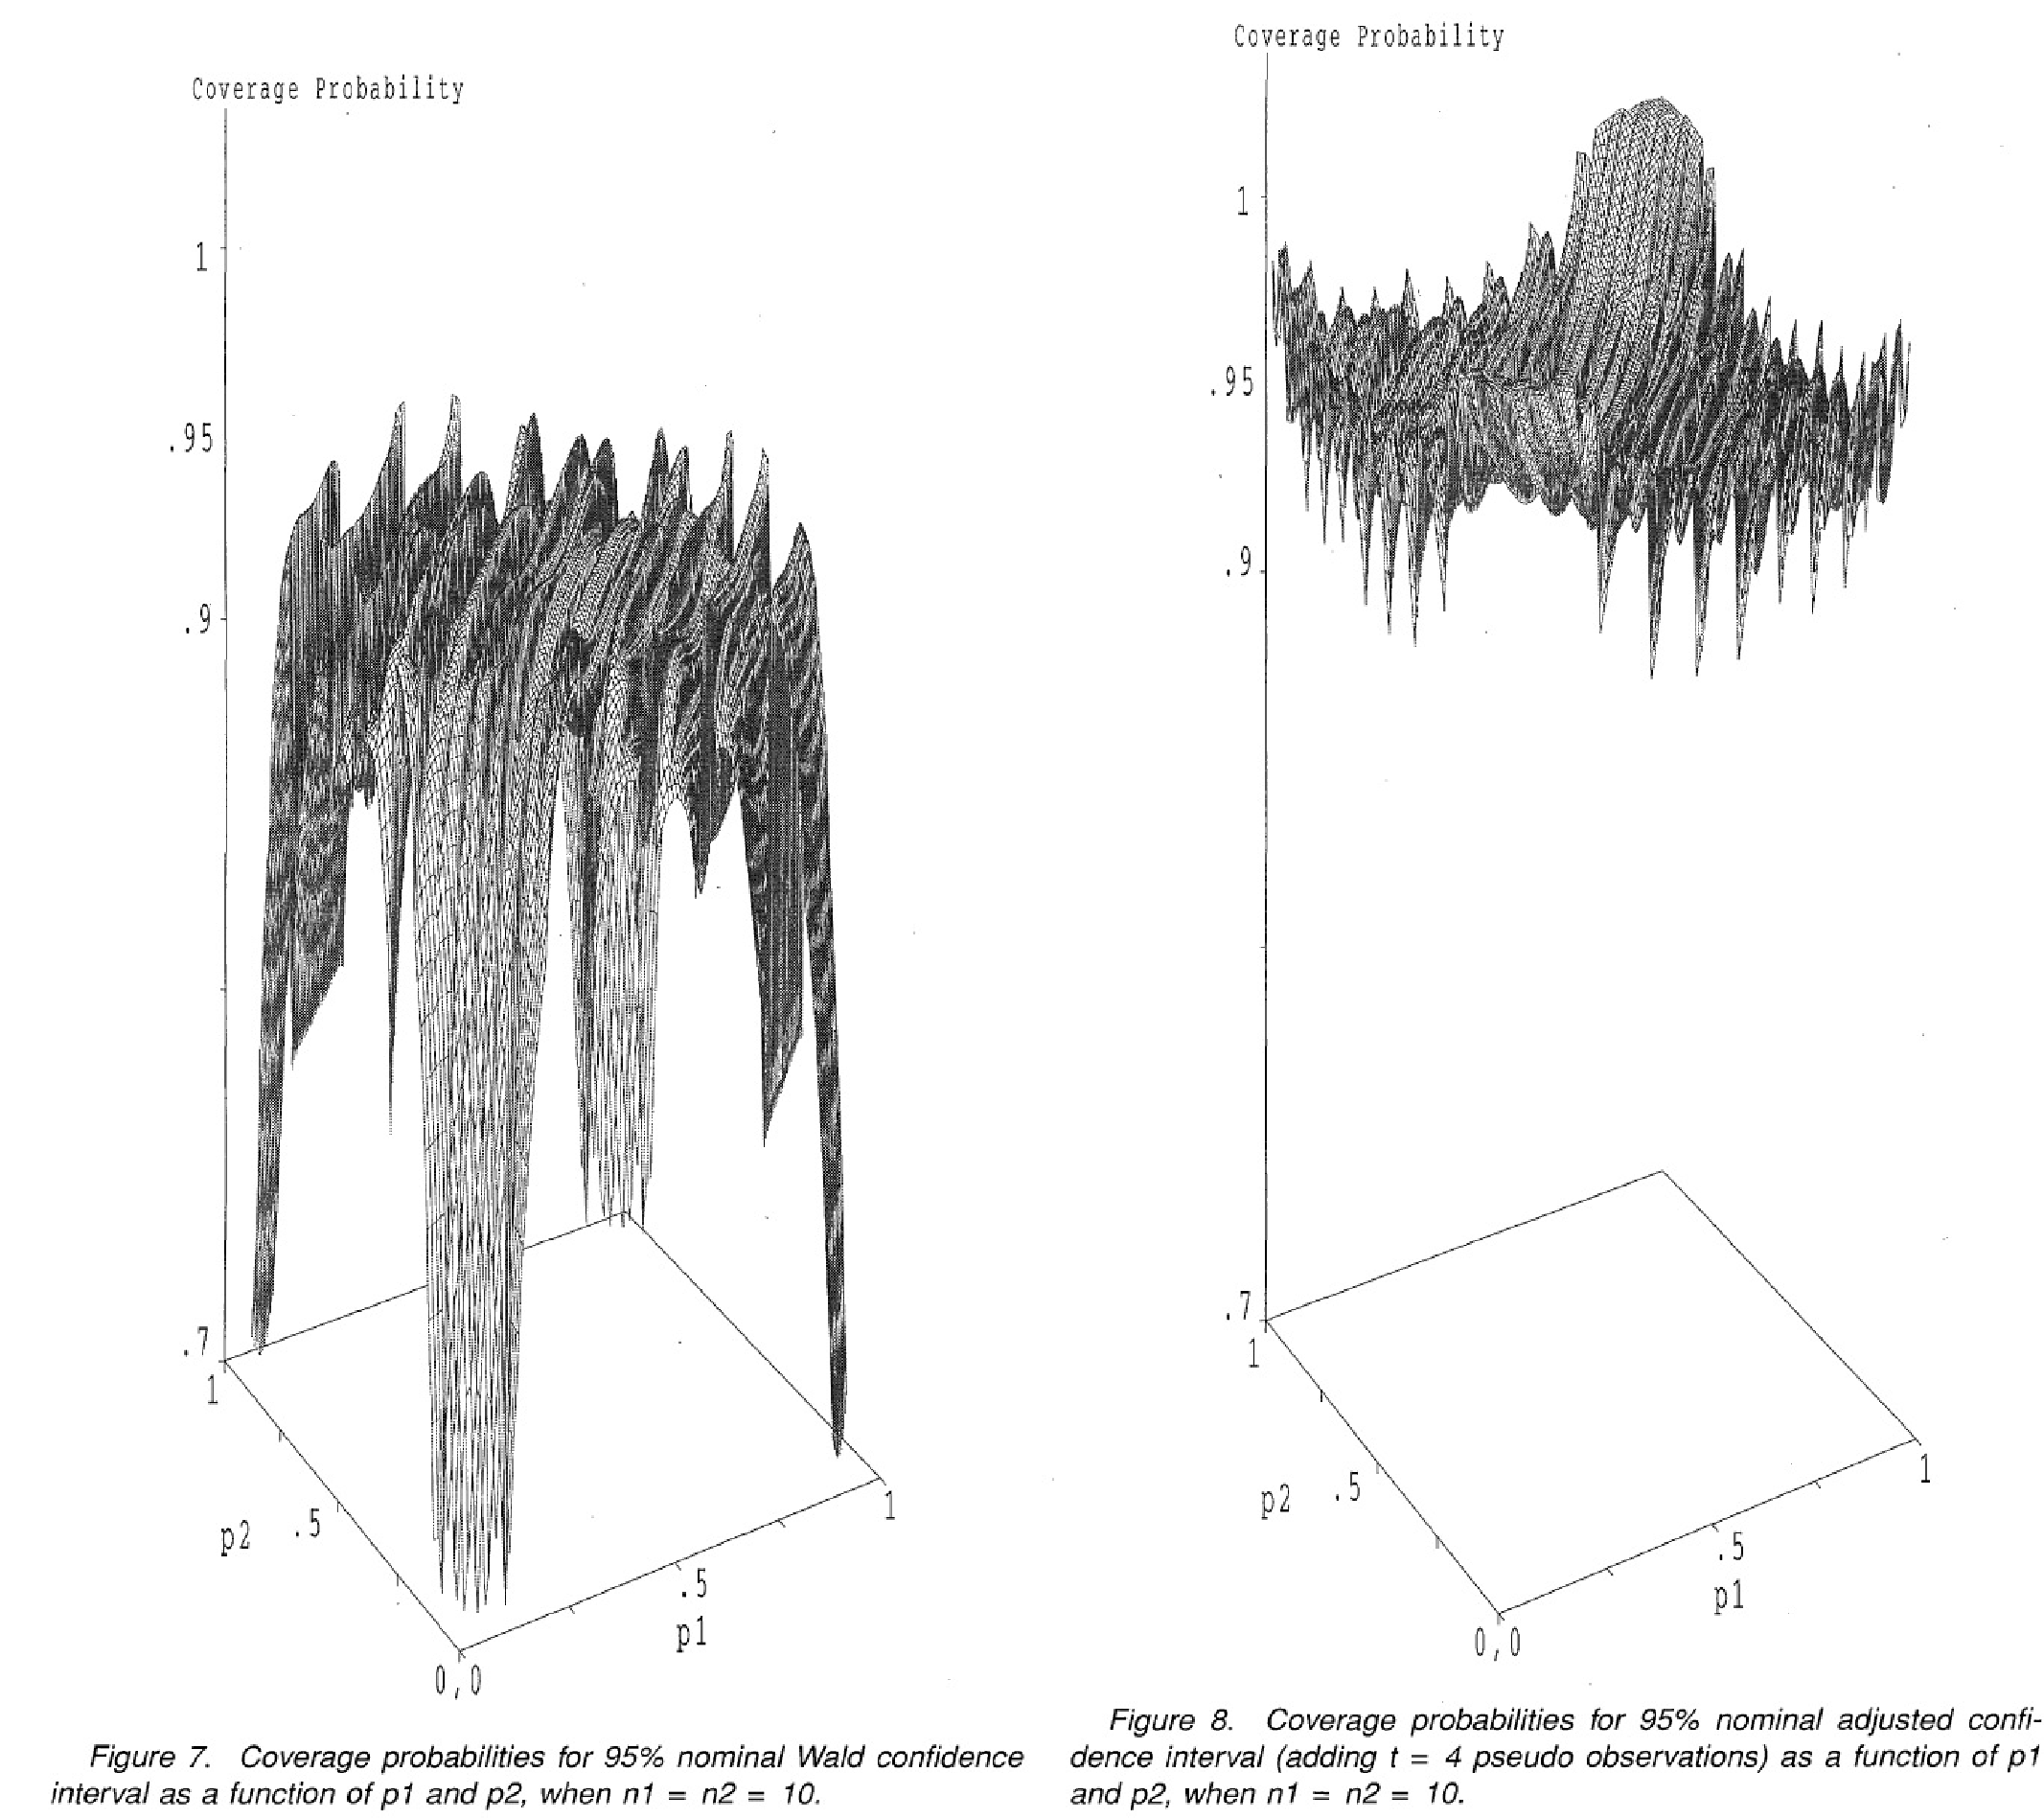
\includegraphics[width=3in]{waldTwoSample2.pdf}
\end{center}
\end{frame}

\begin{frame}\frametitle{Wald versus Agresti /Caffo\footnote{Taken from Agresti and Caffo (2000) TAS }}
\begin{center}
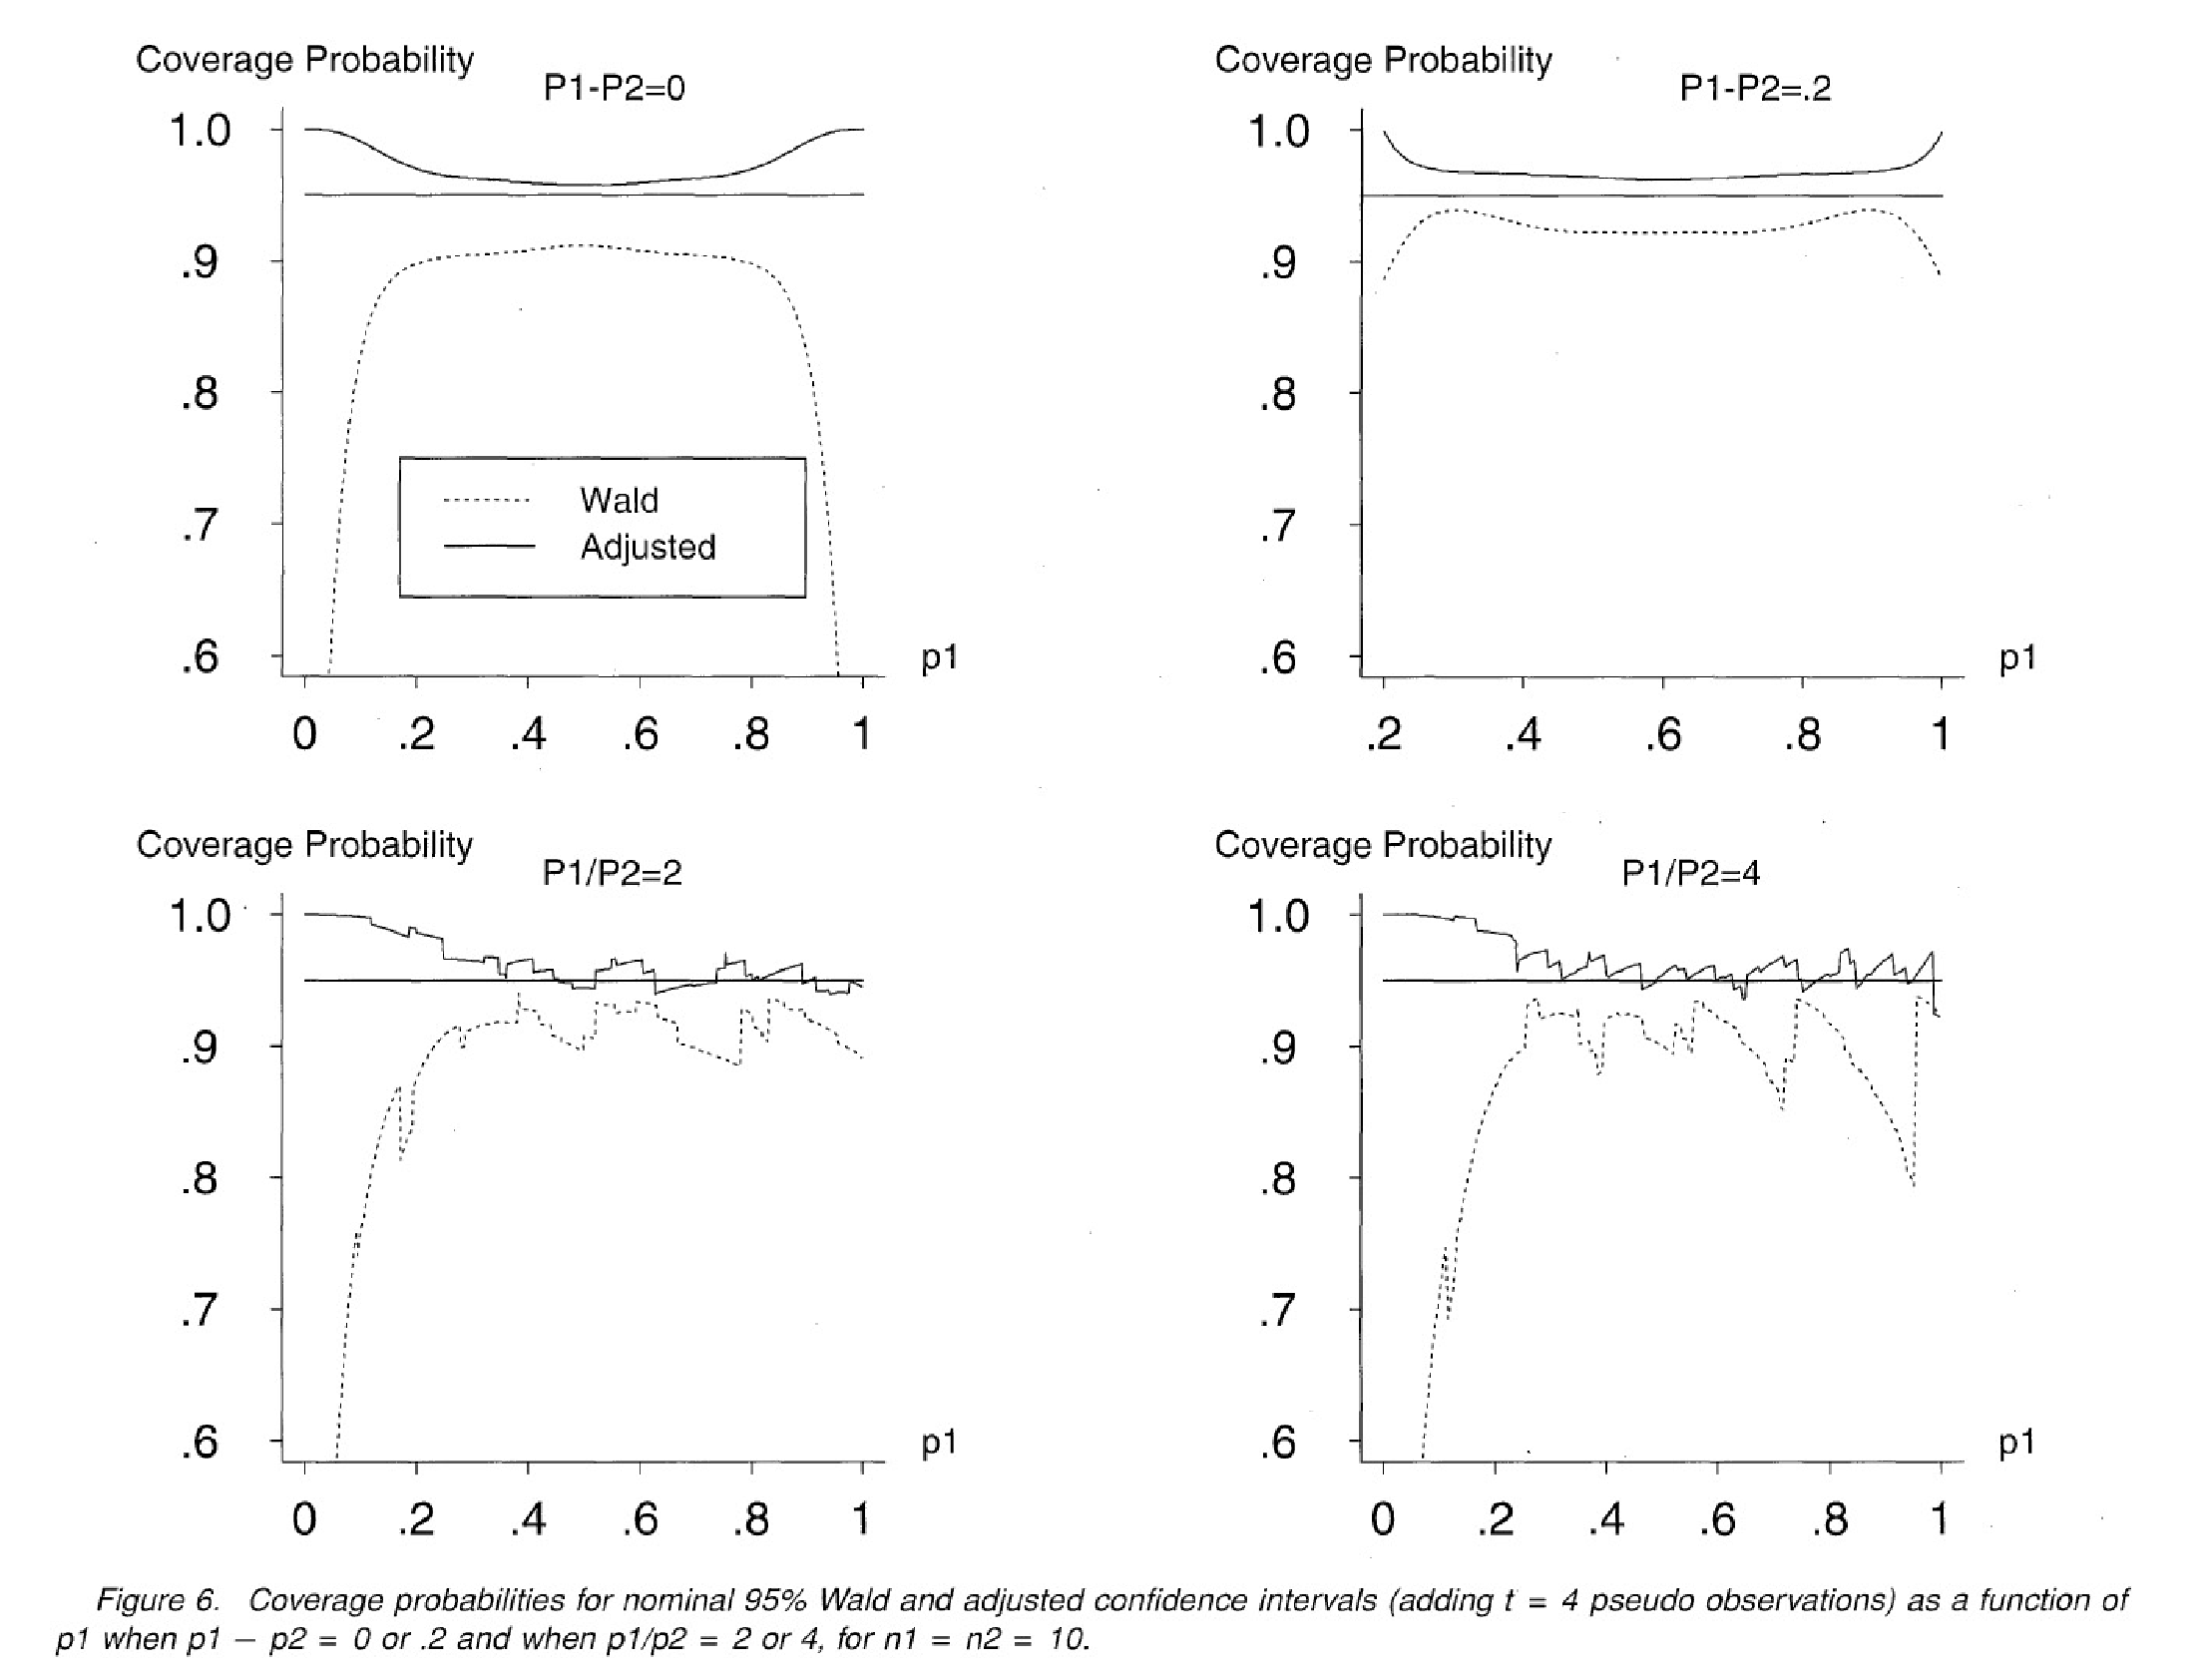
\includegraphics[width=3in]{waldTwoSample.pdf}
\end{center}
\end{frame}

\section{Bayesian and likelihood analysis of two proportions}
\begin{frame}\frametitle{Bayesian and likelihood inference for two binomial proportions}
  \begin{itemize}
  \item Likelihood analysis requires the use of profile likelihoods,
    or some other technique and so we omit their discussion
  \item Consider putting independent Beta$(\alpha_1, \beta_1)$ and Beta$(\alpha_2, \beta_2)$ priors
    on $p_1$ and $p_2$ respectively
  \item Then the posterior is
$$
\pi(p_1, p_2) \propto p_1^{x + \alpha_1 - 1}(1 - p_1)^{n_1 + \beta_1 - 1} \times  p_2^{y+\alpha_2 -1}(1 - p_2)^{n_2+\beta_2-1}
$$
  \item Hence under this (potentially naive) prior, the posterior for $p_1$ and $p_2$ are independent
    betas
  \item The easiest way to explore this posterior is via Monte Carlo simulation
  \end{itemize}
\end{frame}

\begin{frame}[fragile]
\begin{verbatim}
x <- 11; n1 <- 20; alpha1 <- 1; beta1 <- 1
y <-  5; n2 <- 20; alpha2 <- 1; beta2 <- 1
p1 <- rbeta(1000, x + alpha1, n - x + beta1)
p2 <- rbeta(1000, y + alpha2, n - y + beta2)
rd <- p2 - p1
plot(density(rd))
quantile(rd, c(.025, .975))
mean(rd)
median(rd)
\end{verbatim}
\end{frame}

\begin{frame}[fragile]
  \begin{itemize}
  \item The function \texttt{twoBinomPost} on the course web site automates a lot of this
  \item The output is
  \end{itemize}
\begin{verbatim}
Post mn rd (mcse) = -0.278 (0.004)
Post mn rr (mcse) = 0.512 (0.007)
Post mn or (mcse) = 0.352 (0.008)

Post med rd       =  -0.283 
Post med rr       =  0.485 
Post med or       =  0.288 

Post mod rd       =  -0.287 
Post mod rr       =  0.433 
Post mor or       =  0.241 

Equi-tail rd      =  -0.531 -0.008 
Equi-tail rr      =  0.195 0.98 
Equi-tail or      =  0.074 0.966 
\end{verbatim}
\end{frame}

\begin{frame}
  \begin{center}
    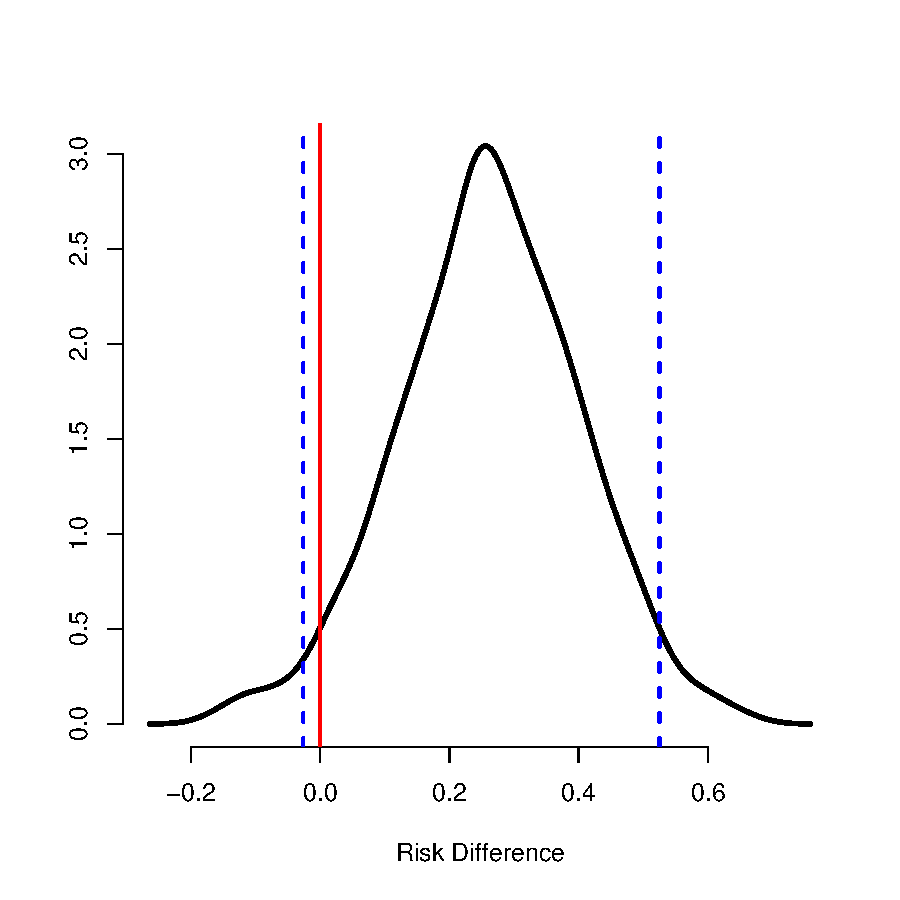
\includegraphics[height=3in]{MCposterior2sampleBinom.pdf}
  \end{center}
\end{frame}
\end{document}

